\section{Evaluation}

\subsection{Rank Lists' Fusions Evaluation \label{sec:eval_fusion}}

In this experiment, the goal is to understand if fusing individual rank lists can create better rank lists.
The methodology used, is to create $n$ isolated rank lists and fuse them for every $r$ rank lists combinations ($C^n_r$ possible rank lists combinations).

The rank list used are the ones obtained by using the $9$ retained rank list methods ($n=9$), see Table~\ref{tab:9rl} in Section~\ref{sec:individual_methods_summary}.
They represent the best configuration retained for each text representation.
The rank list are fused using the two proposed methods: Z-Score fusion and regression fusion.

The $r$ value is selected to $4$, since it represents the number of different text representation.
The number of possible fusion combinations with $n=9$ and $r=4$ is $C^{9}_{4} = 126$.
The 126 resulting fusions rank list are evaluated using the three following metrics: Average Precision (AP), R-Precision (RPrec) and High Precision (HPrec).

To be able to compare the rank list produced by fusion to the non-fused rank lists (one to many), two evaluation strategies are used.
One called \textit{Single-Max} which represent the best metrics for each individual rank list in the fusion and another one called \textit{Single-Mean} which is represented by the mean of each rank list metrics in the fusion.
More information on these two comparison strategy and an example are presented in Section~\ref{sec:evaluation_comparison}.

If the rank lists produced by a fusion overcome the Single-Max evaluation, it means that the resulting rank list give results even better than every individual rank lists used for this fusion.
This represents the best case where the fusion actually improve the results.

If the rank lists produced by a fusion overcome the Single-Mean evaluation, it means that the fused rank list have better results than the expected value of the individual rank lists (when a rank list is selected randomly).
When using the fusions for unsupervised problems (such as clustering), it is a good approach since it gives stability.

For this experiment, the St-Jean A and St-Jean B corpora are used.
The results of every fusion combinations using the proposed rank list and strategies are graphically presented in Figure~\ref{fig:fusions}.

Statistics on the 126 fusions on each metric and fusion schemes are resumed in Tables~\ref{tab:fusion_stats_A}/\ref{tab:fusion_stats_B}.
These tables contain: the minimal value (min), the average and the standard deviation (Avg$\pm$Std), the maximal value, the argmin and argmax for the metrics (using ids of the rank list see Table~\ref{tab:9rl} in Section~\ref{sec:individual_methods_summary}).
The reader can refer to Example~\ref{ex:fusion_eval} to clearly understand the values in these tables.

A sign test between the two strategies and the two fusion methods is presented in Table~\ref{tab:fusion_sign_test}.

Using these metrics on St-Jean, the sign test tends to indicate that the fusion increase the overall quality of the rank list.
The Z-Score fusion, produce for every metrics better results than both Single-Mean and Single-Max, the average precision is increased in average by $\sim 10$\% compared to the average of the average precision (Single-Mean) of the rank list used, and by around 6\% in average when considering the maximal average precision (Single-Max).

In the other hand, the regression fusion, have an average increase of $\sim 3$\% in average precision for the Single-Mean and have a decrease of around $1\%$ when comparing to the Single-Max.
The standard deviation of the regression fusion is greater than the Z-Score fusion, this indicates a slightly greater instability in the results.

A general observation of the Tables~\ref{tab:fusion_stats_A} and \ref{tab:fusion_stats_B} and Figure~\ref{fig:fusions}, show that the HPrec tends to be the least easy metric to increase when using the fusion.
The results of fusing multiple rank lists when using regression fusion strategy tends to indicate that the resulting rank list has in average an equivalent quality as the best rank list used for the fusion, with some slight decreases.
This can be further confirmed by looking at Table~\ref{tab:fusion_B}, line Regression/T/Single-Max contains more ties than other lines.

No particular set of rank list tends to give the best results in every case when fusing with the two strategies.
Every rank list is present in the argmax.
With the Z-Score fusion, the best results are obtained with rank lists using different text representations.
This observation will be further explorer in Section~\ref{sec:fusion_diversity}.

The Z-Score fusion give best results overall.

\begin{example*}
  \caption{Fusion evaluation methodology}
  \label{ex:fusion_eval}

  Imagine a simple scenario where 3 individual rank lists are fused 2 by 2.
  This corresponds to $C^3_2 = 3$ possible fusions combinations.

  \subcaption{Rank lists}
  The three individual rank lists have the following AP evaluation.

  \vspace{0.2cm}

  \begin{center}
    \begin{tabular}{l l}
      \toprule
      Rank lists & AP \\
      \midrule
      Rank list 1 & 0.8 \\
      Rank list 2 & 0.9 \\
      Rank list 3 & 0.7 \\
      \bottomrule
    \end{tabular}
  \end{center}

  \vspace{0.5cm}

  \subcaption{Fusions}
  Now the rank lists are fused using a fusion scheme X.
  These create a single rank list for each rank list combinations.
  They can be evaluated with the average precision.
  For the example, they obtain the score written in column \textit{Fusion X AP} of this following table.

  We can also compute the rank list aggregations using the Single-Mean / Single-Max schemes for each rank list combinations.

  \vspace{0.2cm}

  \begin{center}
    \begin{tabular}{l|l l l}
      \toprule
      Rank lists fusions      & Fusion X AP   & Single-Mean AP   & Single-Max AP\\
      \midrule
      Rank list 1 and 2 & 0.7 & $(0.8 + 0.9) / 2 = 0.85$ & $max(0.8, 0.9) = 0.9$\\
      Rank list 2 and 3 & 0.8 & $(0.9 + 0.7) / 2 = 0.80$ & $max(0.9, 0.7) = 0.9$\\
      Rank list 1 and 3 & 0.9 & $(0.8 + 0.7) / 2 = 0.75$ & $max(0.8, 0.7) = 0.8$\\
      \bottomrule
    \end{tabular}
  \end{center}

  \vspace{0.5cm}

  \subcaption{Statistics}
  Then we can compute statistics for all the rank lists combinations (each column from the previous table).

  \vspace{0.2cm}

  \begin{center}
    \begin{tabular}{l|l l l}
      \toprule
      Statistics        & Fusion X AP   & Single-Mean AP  & Single-Max AP\\
      \midrule
      Min               & 0.7         & 0.75            & 0.8 \\
      Mean$\pm$Std      & 0.8$\pm$0.1 & 0.8$\pm$0.05    & 0.87$\pm$0.06 \\
      Max               & 0.9         & 0.85            & 0.9 \\
      Argmin            & [1, 2]      & [1, 3]          & [1, 3] \\
      Argmax            & [1, 3]      & [1, 2]          & [1, 2] \\
      \bottomrule
    \end{tabular}
  \end{center}

  \vspace{0.2cm}

  Instead of only evaluating the average precision, multiple metrics are used for the real experiment (this creates additional columns).
  The values are also presented differently in the real experiment since two fusion strategies are used.

  \vspace{0.5cm}

  \subcaption{Sign Test}
  Each rank lists combination (each line from the fusion table) can be used to create a sign test.
  If the rank list by fusion is better for one combination than Single-Mean, the fusion earn 1 point.
  If the rank list by fusion have the same results as Single-Mean, it is a tie.
  Otherwise, the Single-Mean earn 1 point.

  The same goes for Single-Max.

  Here is the sign test for the example.

  \vspace{0.2cm}

  \begin{center}
    \begin{tabular}{l|l }
      \toprule
      Sign Test                & AP\\
      \midrule
      Fusion X/Tie/Single-Mean & 1/1/1 \\
      Fusion X/Tie/Single-Max  & 1/0/2 \\
      \bottomrule
    \end{tabular}
  \end{center}

\end{example*}


\begin{figure}
  \centering
  \caption{Evaluation of every combination of 4 rank lists' fusions using Z-Score and Regression}
  \label{fig:fusions}

  \subcaption{Testing on St-Jean A (training St-Jean B, for the Regression fusion)}
  \label{fig:fusion_evaluation_A}
  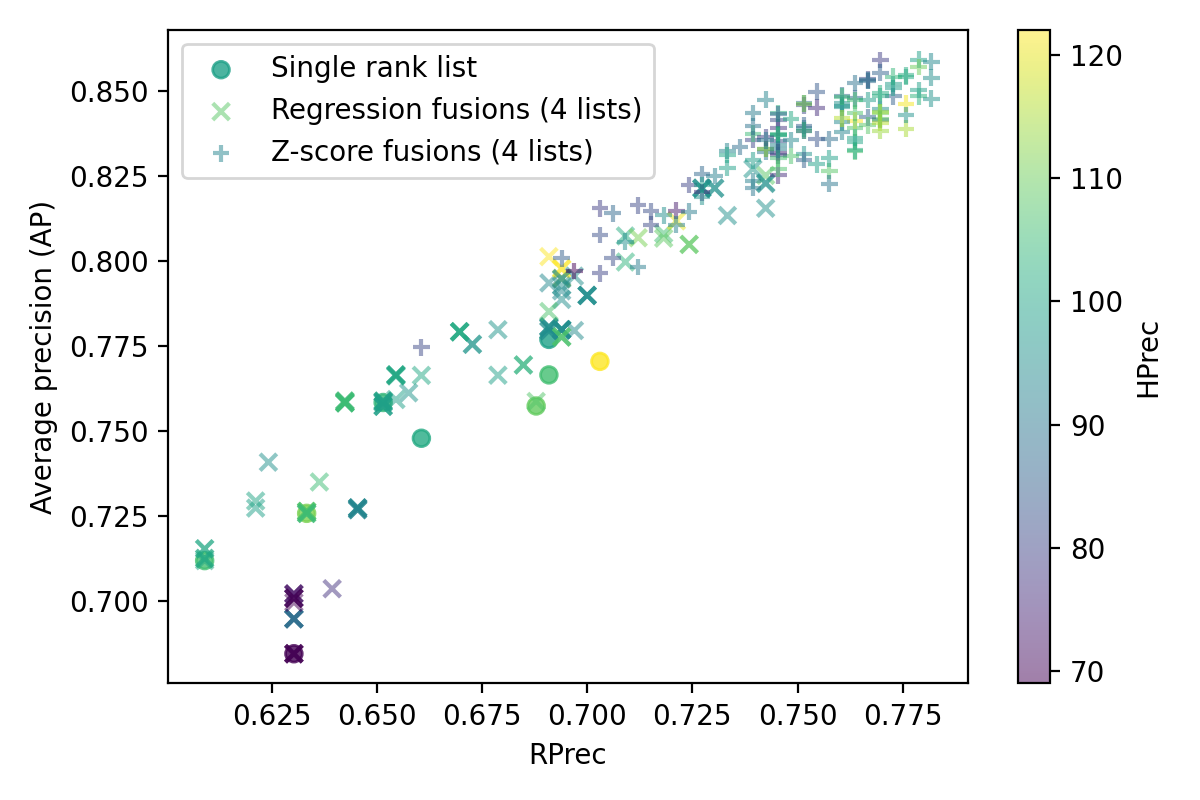
\includegraphics[width=\linewidth]{img/fusion_evaluation_A.png}

  \vspace{0.5cm}

  \subcaption{Testing on St-Jean B (training St-Jean A, for the Regression fusion)}
  \label{fig:fusion_evaluation_B}
  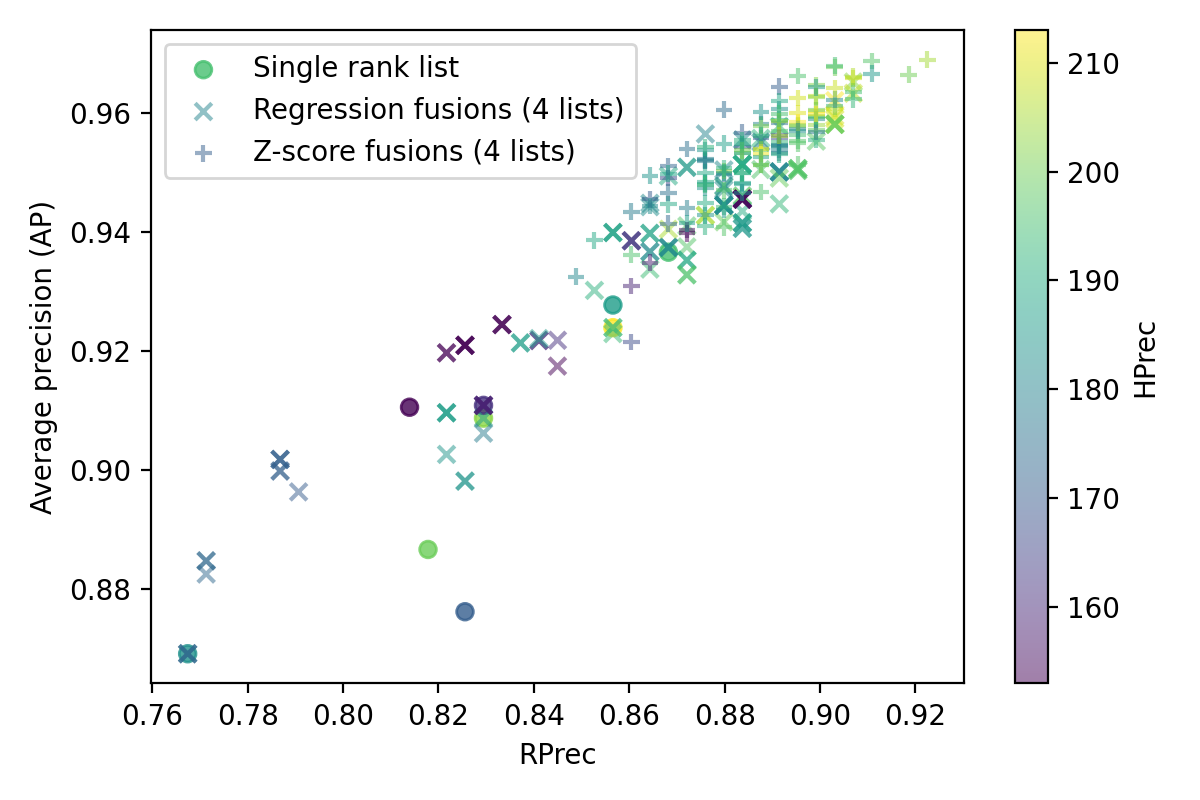
\includegraphics[width=\linewidth]{img/fusion_evaluation_B.png}
\end{figure}

\begin{table}
  \centering
  \caption{Fusion statistics on St-Jean A}
  \label{tab:fusion_stats_A}

  \subcaption{Single-Mean}
  \resizebox{\linewidth}{!}{
  \begin{tabular}{l l l l}
    \toprule
    Stats
    & AP
    & RPrec
    & HPrec \\
    \midrule
    Min & $0.72$ & $0.63$ & $56.25$ \\
    Avg$\pm$Std & $0.74\pm0.01$ & $0.66\pm0.01$ & $70.78\pm8.00$ \\
    Max & $0.77$ & $0.69$ & $84.25$ \\
    Argmin & [1,4,6,7] & [4,5,6,7] & [0,1,5,7] \\
    Argmax & [0,2,5,8] & [0,2,3,8] & [2,3,4,6] \\
    \bottomrule
  \end{tabular}
  }

  \vspace{0.5cm}

  \subcaption{Single-Max}
  \resizebox{\linewidth}{!}{
  \begin{tabular}{l l l l}
    \toprule
    Stats
    & AP
    & RPrec
    & HPrec \\
    \midrule
    Min & $0.75$ & $0.65$ & $72.00$ \\
    Avg$\pm$Std & $0.77\pm0.01$ & $0.69\pm0.01$ & $88.66\pm9.55$ \\
    Max & $0.78$ & $0.70$ & $99.00$ \\
    Argmin & [1,4,6,7] & [4,5,6,7] & [0,1,5,7] \\
    Argmax & [0,1,2,3] & [0,1,2,3] & [0,1,2,3] \\
    \bottomrule
  \end{tabular}
  }

  \vspace{0.5cm}

  \subcaption{Z-Score fusion}
  \resizebox{\linewidth}{!}{
  \begin{tabular}{l l l l}
    \toprule
    Stats
    & AP
    & RPrec
    & HPrec \\
    \midrule
    Min & $0.77$ & $0.66$ & $69.00$ \\
    Avg$\pm$Std & $0.84\pm0.02$ & $0.75\pm0.02$ & $93.92\pm11.15$ \\
    Max & $0.86$ & $0.78$ & $122.00$ \\
    Argmin & [0,4,5,7] & [0,4,5,7] & [0,1,4,5] \\
    Argmax & [0,3,6,7] & [0,3,4,8] & [0,3,7,8] \\
    \bottomrule
  \end{tabular}
  }

  \vspace{0.5cm}

  \subcaption{Regression fusion (training St-Jean B)}
  \resizebox{\linewidth}{!}{
  \begin{tabular}{l l l l}
    \toprule
    Stats
    & AP
    & RPrec
    & HPrec \\
    \midrule
    Min & $0.68$ & $0.61$ & $20.00$ \\
    Avg$\pm$Std & $0.76\pm0.04$ & $0.67\pm0.04$ & $68.84\pm19.41$ \\
    Max & $0.83$ & $0.74$ & $112.00$ \\
    Argmin & [2,3,7,8] & [1,2,4,8] & [2,3,4,7] \\
    Argmax & [0,1,2,6] & [0,1,2,3] & [0,1,3,7] \\
    \bottomrule
  \end{tabular}
  }
\end{table}

\begin{table}
  \centering
  \caption{Fusion statistics on St-Jean B}
  \label{tab:fusion_stats_B}

  \subcaption{Single-Mean}
  \resizebox{\linewidth}{!}{
  \begin{tabular}{l l l l}
    \toprule
    Stats
    & AP
    & RPrec
    & HPrec \\
    \midrule
    Min & $0.89$ & $0.81$ & $137.50$ \\
    Avg$\pm$Std & $0.91\pm0.01$ & $0.83\pm0.01$ & $154.89\pm7.22$ \\
    Max & $0.92$ & $0.85$ & $172.00$ \\
    Argmin & [3,4,6,8] & [1,3,6,8] & [1,6,7,8] \\
    Argmax & [0,2,5,7] & [0,2,5,7] & [0,3,4,5] \\
    \bottomrule
  \end{tabular}
  }

  \vspace{0.5cm}

  \subcaption{Single-Max}
  \resizebox{\linewidth}{!}{
  \begin{tabular}{l l l l}
    \toprule
    Stats
    & AP
    & RPrec
    & HPrec \\
    \midrule
    Min & $0.91$ & $0.83$ & $153.00$ \\
    Avg$\pm$Std & $0.93\pm0.01$ & $0.86\pm0.01$ & $174.75\pm7.29$ \\
    Max & $0.94$ & $0.87$ & $182.00$ \\
    Argmin & [3,4,6,8] & [1,3,6,8] & [1,6,7,8] \\
    Argmax & [0,1,2,3] & [0,1,2,3] & [0,1,2,5] \\
    \bottomrule
  \end{tabular}
  }

  \vspace{0.5cm}

  \subcaption{Z-Score fusion}
  \resizebox{\linewidth}{!}{
  \begin{tabular}{l l l l}
    \toprule
    Stats
    & AP
    & RPrec
    & HPrec \\
    \midrule
    Min & $0.92$ & $0.85$ & $153.00$ \\
    Avg$\pm$Std & $0.95\pm0.01$ & $0.89\pm0.01$ & $188.91\pm12.87$ \\
    Max & $0.97$ & $0.92$ & $213.00$ \\
    Argmin & [2,3,6,8] & [3,4,6,8] & [1,2,3,6] \\
    Argmax & [1,2,5,7] & [1,2,5,7] & [0,3,4,7] \\
    \bottomrule
  \end{tabular}
  }

  \vspace{0.5cm}

  \subcaption{Regression fusion (training St-Jean A)}
  \resizebox{\linewidth}{!}{
  \begin{tabular}{l l l l}
    \toprule
    Stats
    & AP
    & RPrec
    & HPrec \\
    \midrule
    Min & $0.87$ & $0.77$ & $124.00$ \\
    Avg$\pm$Std & $0.93\pm0.02$ & $0.86\pm0.04$ & $165.25\pm22.09$ \\
    Max & $0.97$ & $0.91$ & $210.00$ \\
    Argmin & [2,3,6,8] & [2,3,6,8] & [1,2,3,8] \\
    Argmax & [0,1,2,7] & [0,1,2,7] & [0,1,3,7] \\
    \bottomrule
  \end{tabular}
  }
\end{table}

\begin{table*}
  \centering
  \caption{Rank lists' fusion sign test. \textit{The star (*) indicate a Binomial test p-value smaller than 5\%}}
  \label{tab:fusion_sign_test}

  \subcaption{Testing St-Jean A (training St-Jean B, for the Regression fusion)}
  \label{tab:fusion_A}
  \begin{tabular}{l c c c}
    \toprule
    Metric
    & AP
    & RPrec
    & HPrec \\
    \midrule
    Z-Score/Tie/Single-Mean    & *126/0/0 & *126/0/0 & *124/0/2 \\
    Z-Score/Tie/Single-Max     & *125/0/1 & *124/1/1 & *77/4/45 \\
    Regression/Tie/Single-Mean & *85/0/41 & 66/1/59  & 58/1/67  \\
    Regression/Tie/Single-Max  & 58/0/68  & 38/7/81* & 16/5/105* \\
    \bottomrule
  \end{tabular}

  \vspace{0.5cm}

  \subcaption{Testing St-Jean B (training St-Jean A, for the Regression fusion)}
  \label{tab:fusion_B}
  \begin{tabular}{l c c c c}
    \toprule
    Metric
    & AP
    & RPrec
    & HPrec \\
    \midrule
    Z-Score/Tie/S-Mean    & *126/0/0  & *126/0/0  & *126/0/0 \\
    Z-Score/Tie/S-Max     & *125/0/1  & *123/2/1  & *108/2/16\\
    Regression/Tie/S-Mean & *116/0/10 & *103/1/22 & *87/1/38 \\
    Regression/Tie/S-Max  & *87/0/39  & *72/11/43 & 43/9/74* \\
    \bottomrule
  \end{tabular}

\end{table*}

\subsection{Veto Evaluation}

In this experiment, the goal is to understand if the veto method can improve the average precision on the fused rank lists when using the regression fusion method.
To do so, the St-Jean retained rank list are used (ref. Table~\ref{tab:rls_st_jean} in annex).
The fusion scheme is learnt on first St-Jean A and trained on St-Jean B (ref. Section~\ref{sec:regression_fusion}), then inversely.

After computing the probabilities for each link in each rank list on the testing set, the probabilities under the threshold are set according to each proposed veto strategy (set to $0$, $-1$, $-n$, $-\infty$).

An evaluation is done for the threshold ranging between $0.01$ and $0.50$, with a step of $0.01$.
A threshold of $0.50$ is a theoretical upper bound.
After a threshold of $0.50$, the false link probability is smaller than the true link probability.
Having a veto on a link more likely to be true link than false link is a bad idea.

Rank lists' regression fusion are normally computed with the probabilities average, with one small difference for the $-\infty$ strategy when a $-\infty$ is encountered in the mean, the mean will always be $-\infty$.
To understand if the veto improve the results, the average precision gain is compute between the rank list with and without the veto strategy.

The average precision gain over the threshold value is visually presented in Figure~\ref{fig:veto}.
The best configurations found are summarized in Table~\ref{tab:veto}.

Overall, the veto strategy seem to be a bad option.
The best result obtained have only a $0.0193$ gain in average precision, with a threshold of $0.01$, which is the closest to the non threshold approach, since only a small portion of the rank list is affected.
This tiny improvement may be due to random factors.
Using the $-\infty$ strategy only give worse results.

The veto strategy is only impactful when most of the rank lists rank a false link at the top, except one rank list which correctly identify this false link and rank him at the bottom.
The rank list used for the experiment do not have such special case, since most of them correct classify false link at the bottom and true links at the top.
This can be one possible reason on why the veto fail to improve the results.
This strategy may be appliable on harder corpus such as the PAN 16 corpus or with even more diverse rank list generation strategies.

\begin{figure}
  \caption{Veto strategies evaluations on St-Jean A and B depending on the threshold}
  \label{fig:veto}
  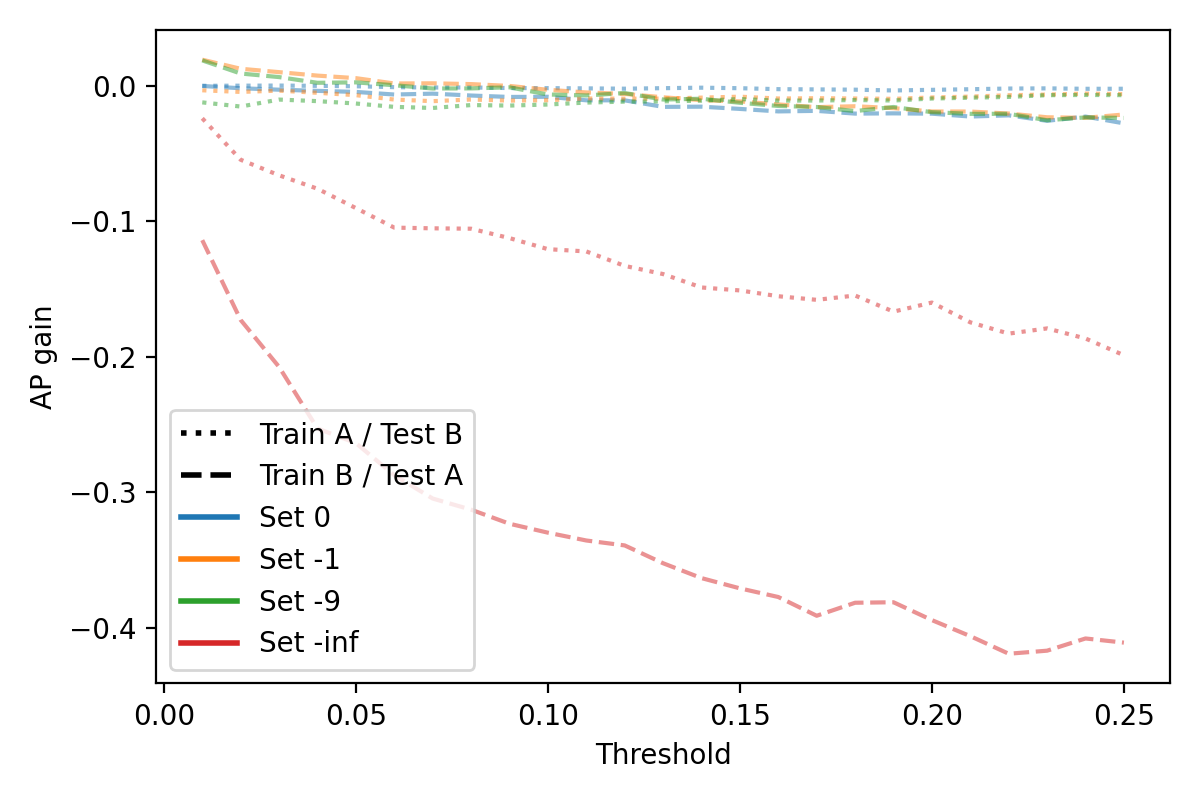
\includegraphics[width=\linewidth]{img/veto.png}
\end{figure}

\begin{table}
  \centering
  \caption{Maximal gain on the average precision using the veto / Argmax}
  \label{tab:veto}
  \begin{tabular}{l c c}
    \toprule
                   & \multicolumn{2}{c}{Train/Test} \\
                   & A/B            & B/A \\
    \midrule
    Set to $0$     & 1.98e-04/0.03  & -9.11e-05/0.01 \\
    Set to $-1$    & -3.28e-03/0.01 & 1.93e-02/0.01 \\
    Set to $-n$    & -6.73e-03/0.24 & 1.88e-02/0.01 \\
    Set to $-\inf$ & -2.40e-02/0.01 & -1.14e-01/0.01 \\
    \bottomrule
  \end{tabular}
\end{table}

\subsection{Soft-veto Evaluation}

To evaluate the soft veto strategy performances, the same strategy as for the veto strategy is used.
The average precision gain obtained when using the soft-veto over the fusion without veto is computed.
The Z-Score fusion strategy is used for this experiment.

The soft-veto has two parameters: $c$ and $r$, to be able to find the best parameters the grid search approach is used.
Since the $c$ parameter must be in the interval $\left]0, \infty\right[$ and the $r$ parameter must be in the interval $\left]0, \infty\right[$, the grid is constructed from the Cartesian product of the two following sets.
$c = \left\{0 + \epsilon, 1, 2, ..., 19, 20\right\}$, with $\epsilon$ a small value (for example $10^{-6}$) and $r = \left\{0.10, 0.14, ..., 0.86, 0.90\right\}$.
When computing the soft-veto gain using the grid search on the retained rank lists from Oxquarry (see Table~\ref{tab:9rl}), Figure~\ref{fig:soft_veto} is obtained.

The best parameters are $c=18$ and $r=0.14$ with an average precision gain of $3.50e-04$.
Like for the veto experiment, no real average precision gain can be obtained using the soft-veto strategy.
The average precision gain is small and can be due to random factors.

\begin{figure}
  \caption{Average precision gain with soft veto s-curve on Oxquarry}
  \label{fig:soft_veto}
  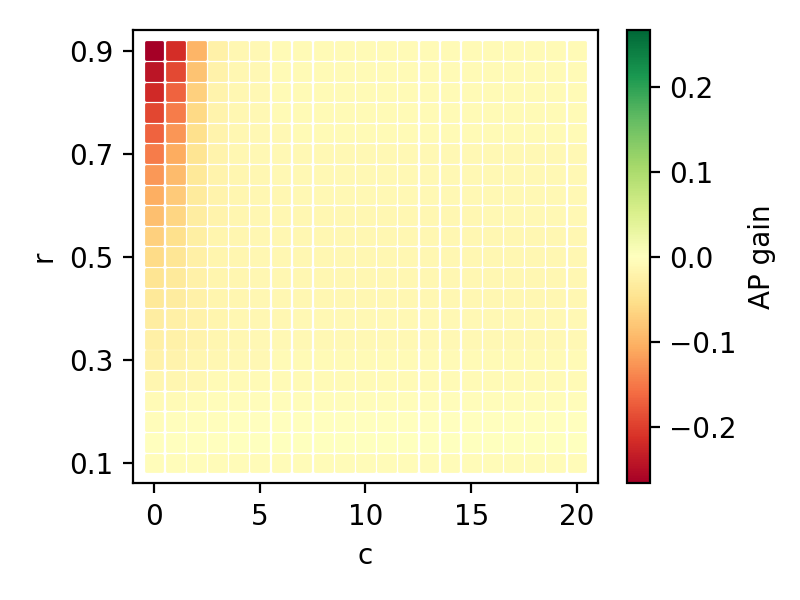
\includegraphics[width=\linewidth]{img/soft_veto.png}
\end{figure}

\subsection{Average Precision Fusion Gain Relation with the Rank Lists Diversity \label{sec:fusion_diversity}}

As stated previously, we believe fusing high quality rank lists (high AP), with the most diverse results can increase the quality of the rank list obatined by fusion.
In this section, we aim to provide even more clues to motivate this assumption.
First, a correlation metric to compare the rank lists must be selected.
Secondly, we compare the correlation coefficients to the average precision gain to verify the assumption.

To compute a correlation between two rank lists, the Kendall rank correlation coefficient is used \cite{scipy}.
The Kendall rank correlation computes a correlation index based on the ordinal association between the two rank lists by computing the number of swaps needed to obtain one rank list from the other.
The fewer swaps needed, the closer the rank lists are.

The default weighing strategy called \textit{hyperbolic weighing} is used for the Kendall rank correlation coefficient.
It favours top ranks in the same fashion as the reciprocal rank ($1 / (r + 1)$).
Swaping top ranks are more important for the Kendall coefficient than bottom ranks.

The Kendall coefficient is ranged between -1 and 1, with 1 being an identical correlation and -1 a completely different correlation.
If our assumption is correct, the average precision gain obtained by fusing two rank lists should be negatively correlated to the rank list Kendall correlation coefficient.
A large gain, when the rank lists are different, thus a low rank list correlation coefficient, and vice versa.

The fusion strategy used here is the Z-Score fusion, since this strategy is parameterless and obtained satisfying results during previous experiments.
As for previous experiments dealing with fusion, the gain in average precision when comparing a set of rank list to a fused rank list can be established in the two following ways: \textit{Single-Mean} and \textit{Single-Max}.
Single-Mean represent the rank lists' mean average precision and Single-Max the rank list maximal average precision.
Example~\ref{ex:gain} in Section~\ref{sec:evaluation_comparison} contain a small example with two rank lists for the Single-Mean and Single-Max methods to compute the average precision gain.

Table~\ref{tab:rl_correlations} show the Kendall correlation coefficient for every pairwise rank lists combination in St-Jean (retained rank lists, see Table~\ref{tab:9rl} in Section~\ref{sec:individual_methods_summary}).

The most similar rank lists pair are the two rank list using letters $n$-grams (0.95).
This result can be easily understood, since both rank list use a similar text representation and distance measure.
They thus obtain similar rank lists.

The least similar rank lists pair are the BZip2 compression and the $250$-MF $2$-POS (0.66).
The compression method is the simplest approach, this method does not require to understand the text to create the rank list.
As for the $250$-MF $2$-POS rank list, to create the rank list, it requires two level of understanding.
First the parser need to understand texts to create the POS, and the second level are the short sequences which involve an even deep understanding of the text.
Due to this large difference in rank list construction, the two rank lists obtain a small correlation coefficient.

For every pair of retained rank lists in St-Jean, the Single-Mean fusion gain is computed and is compared to the correlation coefficient in Figure~\ref{fig:rl_correlations}.
Using the linear regression, the best line for these point is computed \cite{scipy}.
After reproducing this experiment for every corpus and fusion gain computation methods, the results in Table~\ref{tab:rl_correlations_regression} are obtained.

For all experiment the linear correlation coefficient, $r$-value, is negative, which indicate that the average precision gain is negatively correlated to the Kendall correlation coefficient between the rank lists.
Thus, the assumption that suggested that the more diverse the rank lists are, the higher the quality of the fusion, seem to be confirmed.
The $p$-value for the linear regression (null hypothesis: the slope is 0) obtained after the regression is below 5\% for every of the Single-Mean experiments and for the Single-Max St-Jean corpus.
A clear linear relationship between the average precision gain and rank list diversity is observed.

Using the Single-Max strategy on Oxquarry and Brunet give a p-value of 15.1\% and 7.04\% respectively.
This can indicate that the linear correlation between the average precision gain and the diversity of the rank list can be due to random factors.

Since the Single-Mean average precision gain follow a linear model, the gain can be predicted using the slope and the y-intercept of the linear regression.
In an unsupervised model, computing the Kendall correlation coefficient can allow to optimize the fusion gain.
The lowest the correlation coefficient, the greater the average precision gain should be.

This approach have one main draw back.
The rank list used have to be known has \textit{good rank list}.
Otherwise, if a \textit{bad rank list} and a \textit{good rank list} are compared using Kendall correlation coefficient, they will obtain a low correlation, since \textit{bad answers} are often very different from \textit{good answers}.
This low correlation coefficient should indicate a positive good gain.
But when fused, the gain will not be positive, since fusing \textit{bad rank lists} and \textit{good rank lists} tends to produce terrible results.

\begin{table}
  \centering
  \caption{Pairwise Kendall correlation coefficient on St-Jean retained rank lists}
  \label{tab:rl_correlations}
  \resizebox{\linewidth}{!}{
  \begin{tabular}{r|r r r r r r r r}
    \toprule
    id &    1 &    2 &    3 &    4 &    5 &    6 &    7 &    8 \\
    \midrule
    0  & 0.86 & 0.83 & 0.80 & 0.88 & 0.91 & 0.73 & 0.81 & 0.75 \\
    1  &    - & 0.87 & 0.83 & 0.80 & 0.83 & 0.79 & 0.73 & 0.77 \\
    2  &    - &    - & 0.84 & 0.78 & 0.80 & 0.82 & 0.72 & 0.79 \\
    3  &    - &    - &    - & 0.78 & 0.81 & 0.80 & 0.75 & 0.85 \\
    4  &    - &    - &    - &    - & 0.95 & 0.77 & 0.81 & 0.75 \\
    5  &    - &    - &    - &    - &    - & 0.78 & 0.82 & 0.77 \\
    6  &    - &    - &    - &    - &    - &    - & 0.66 & 0.79 \\
    7  &    - &    - &    - &    - &    - &    - &    - & 0.82 \\
    \bottomrule
  \end{tabular}
  }
\end{table}

\begin{figure}
  \centering
  \caption{Fusion average precision gain (using Single-Mean scheme) over rank list distance on St-Jean}
  \label{fig:rl_correlations}
  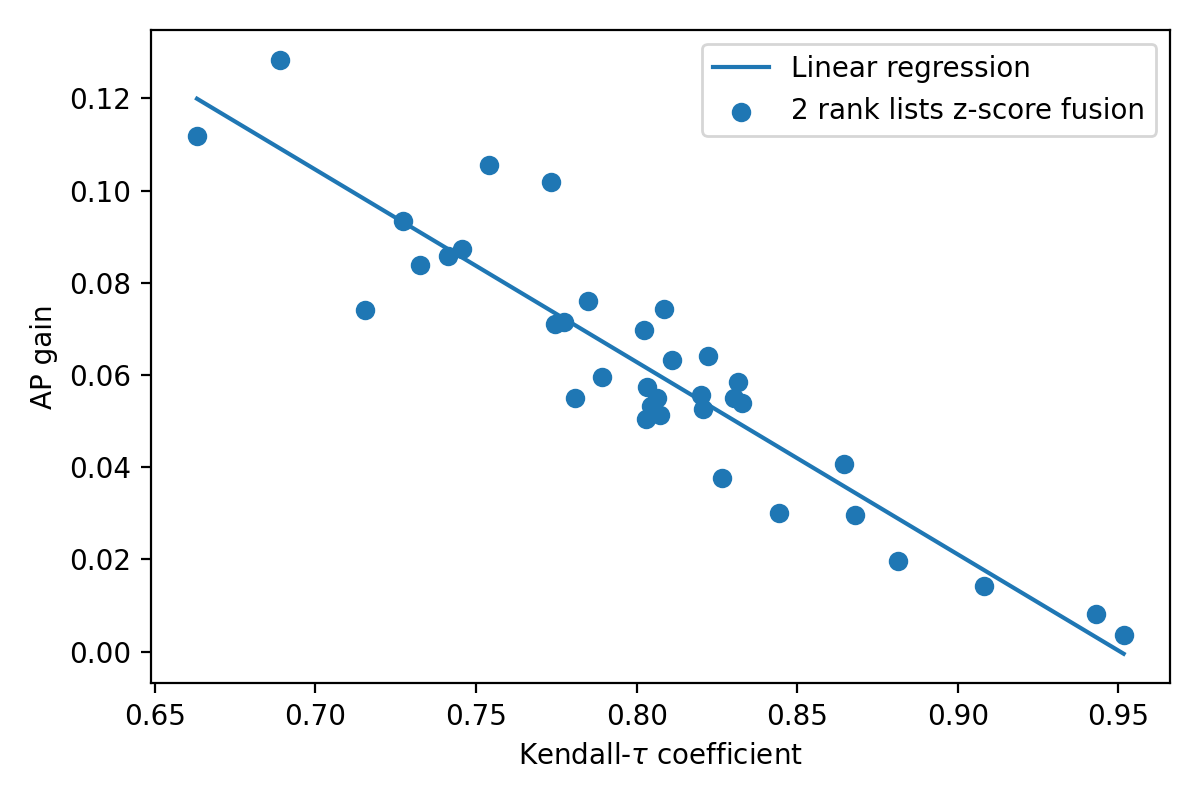
\includegraphics[width=\linewidth]{img/rank_list_correlation_mean_st_jean.png}
\end{figure}

\begin{table}
  \centering
  \caption{Linear regression on the average precision gain over Kendall r-coefficient}
  \label{tab:rl_correlations_regression}

  \subcaption{Single-Mean}
  \begin{tabular}{l r r r r r}
    \toprule
    Corpus/Method & $r$-value & $p$-value & Std. error \\
    \midrule
    Oxquarry & -0.63 & 2.04e-03 & 4.36e-02 \\
    Brunet   & -0.89 & 7.14e-08 & 2.17e-02 \\
    St-Jean  & -0.93 & 9.30e-17 & 2.49e-02 \\
    \bottomrule
  \end{tabular}

  \vspace{0.5cm}

  \subcaption{Single-Max}
  \begin{tabular}{l r r r r r}
    \toprule
    Corpus/Method & $r$-value & $p$-value & Std. error \\
    \midrule
    Oxquarry  & -0.32 & 1.51e-01 & 8.15e-02 \\
    Brunet    & -0.40 & 7.04e-02 & 4.50e-02 \\
    St-Jean   & -0.86 & 1.60e-11 & 3.72e-02 \\
    \bottomrule
  \end{tabular}
\end{table}
